\section{Restructuring}
\label{sec:Restructuring}

After specifying the interfaces of all components, the subsystem decomposition needs to be restructured to reflect all changes. Regarding the generation of code in various programming languages, we identified that the \texttt{Migration} \texttt{Manager} and \texttt{Library} \texttt{Generation} subsystems require the same functionality. As a result, a \texttt{Code} \texttt{Generation} subsystem was extracted that provides its service to the \texttt{Migrator} component and the \texttt{IDL} \texttt{Conversion} subsystem. By that no redundant functionality has to be implemented. 

Additionally, we decided to use JavaScript for handling convert and revert operations defined in \texttt{Replace\-Changes}. Therefore, the \texttt{Source\-Code} \texttt{Importer} subsystem must support parsing it. The restructured subsystem decomposition is illustrated in Figure \ref{fig:subsystemRestructured}.

\begin{figure}[!h]
	\centering{
		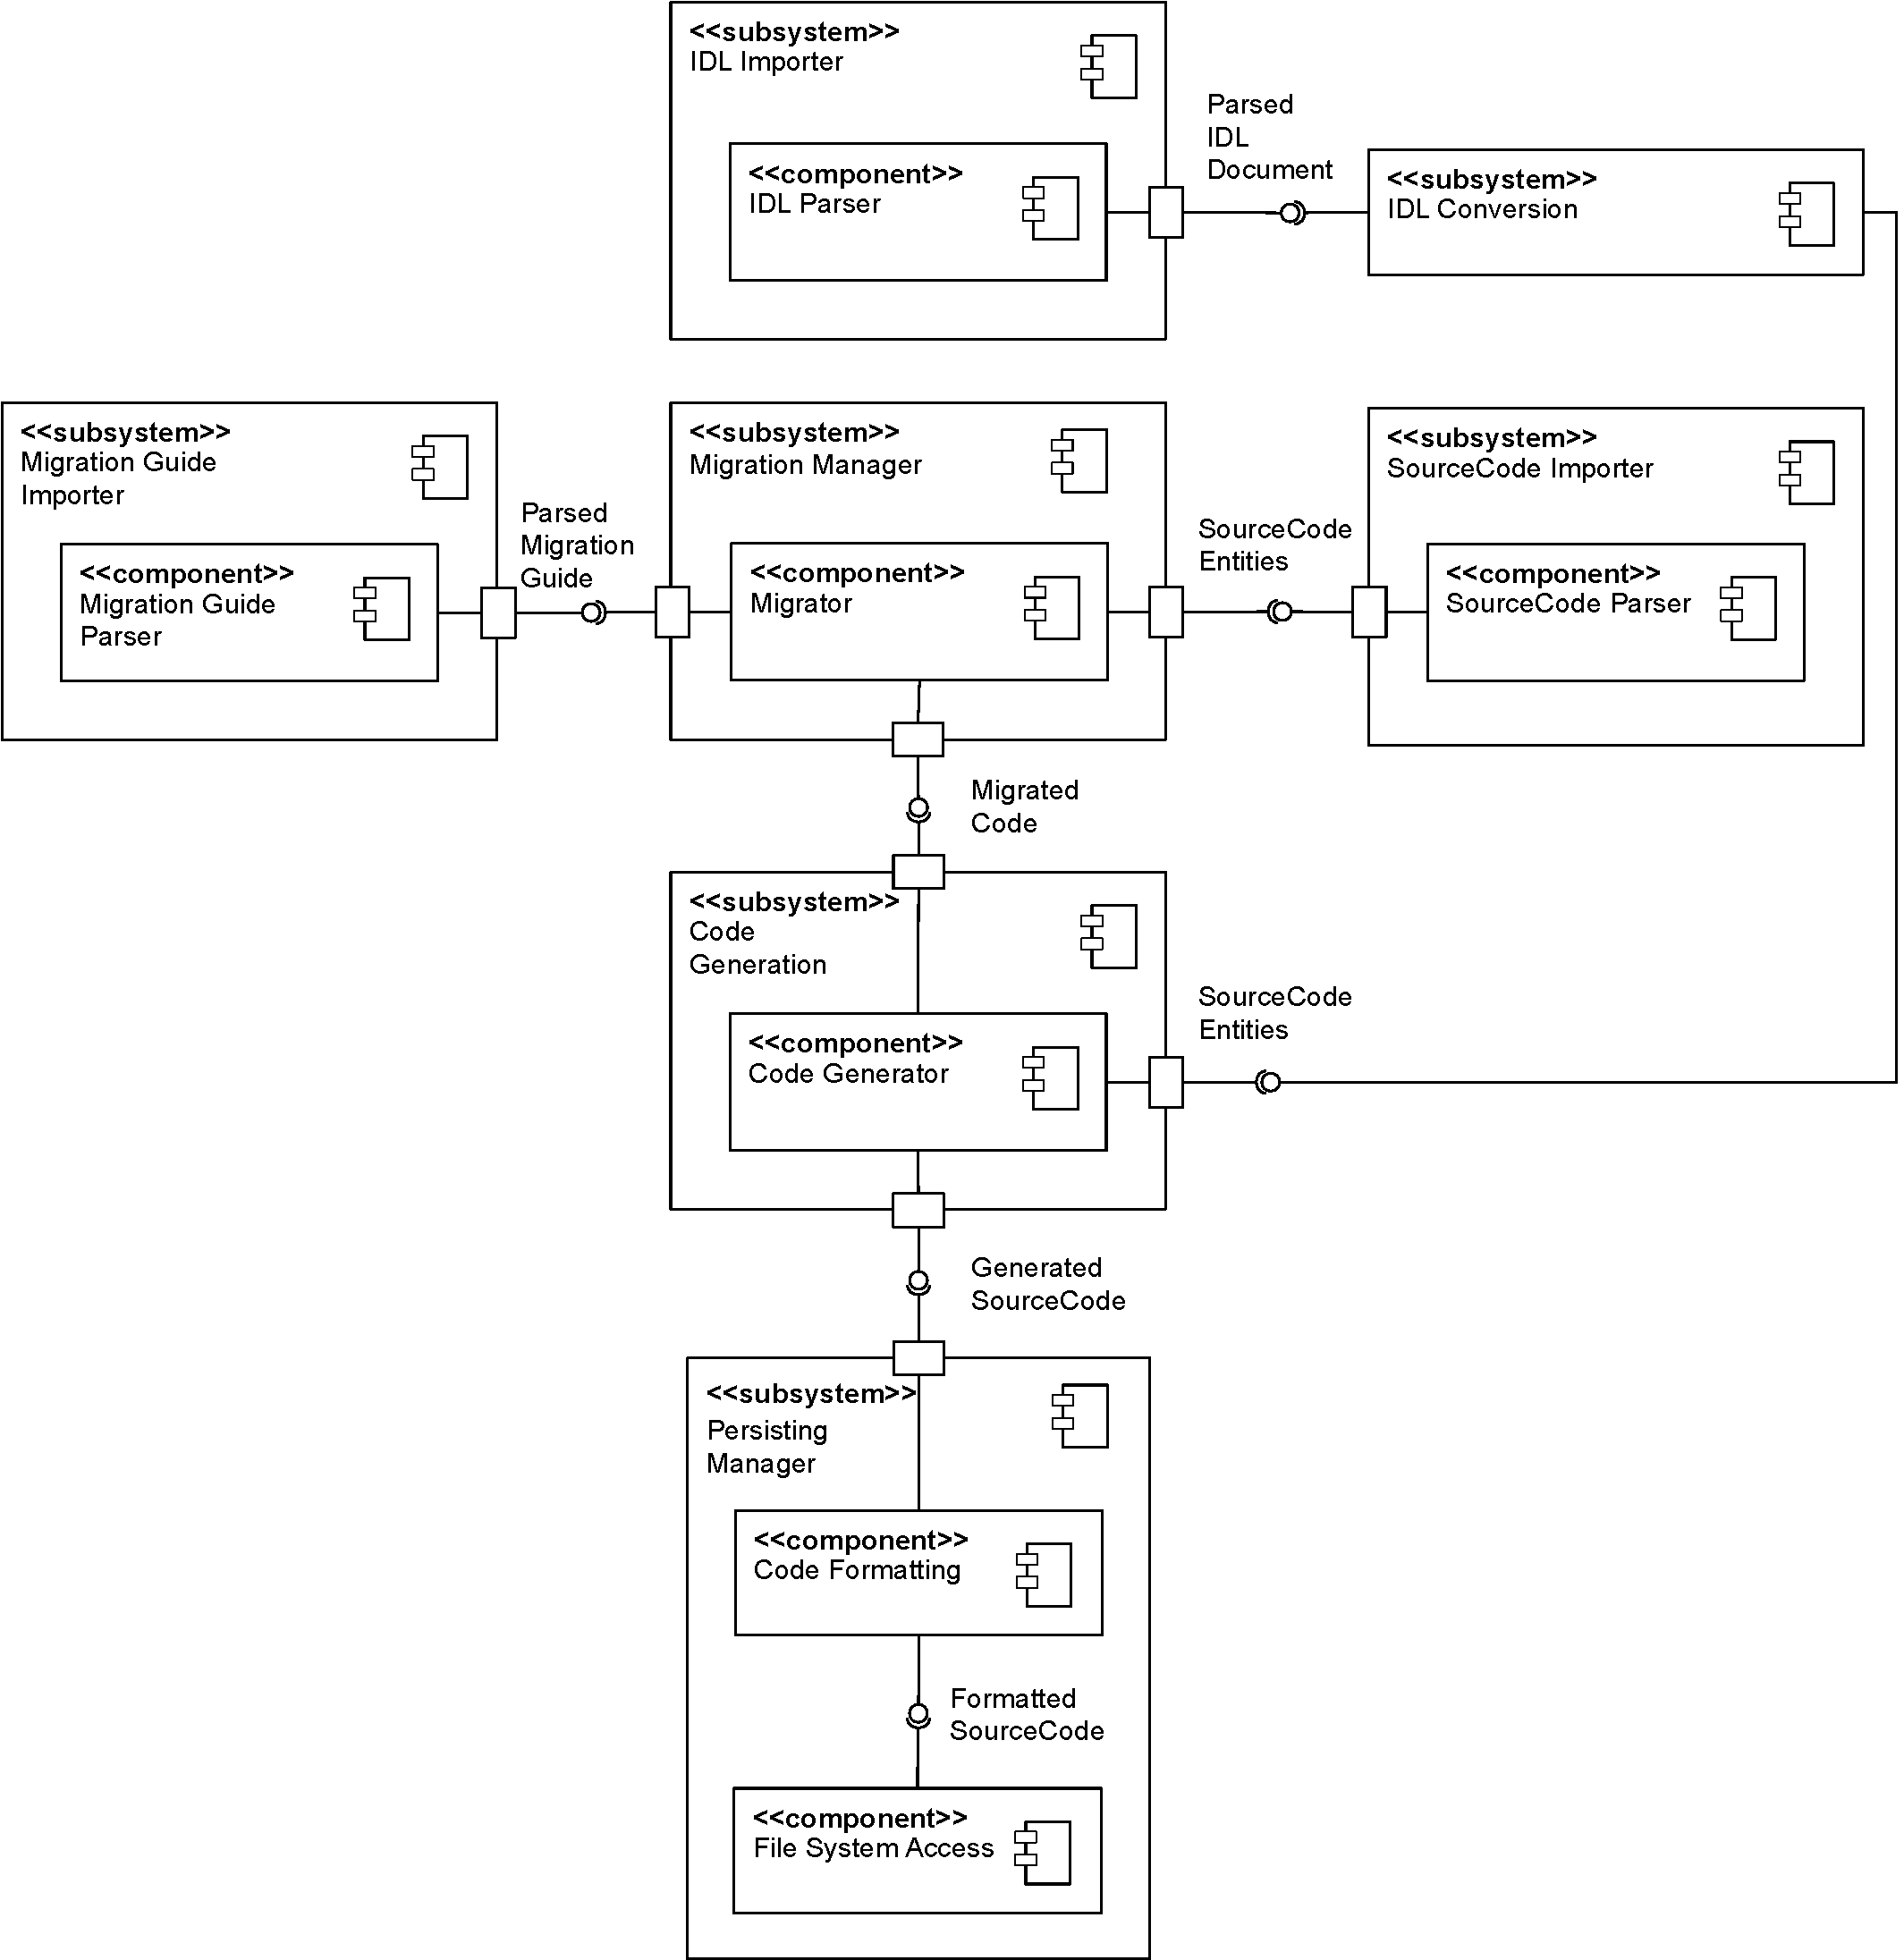
\includegraphics[width=155mm]{images/subsystem_restructured.pdf}
		\caption[Restructured subsystem decomposition]{Restructured subsystem decomposition - The \texttt{Code Generation} subsystem was extracted from the \texttt{Migration Manager} and \texttt{Library Generation} subsystems to provide a uniform interface to both subsystems}
		\label{fig:subsystemRestructured}
	}
\end{figure}